\documentclass[a4paper,12pt]{article}

% ── Packages ──────────────────────────────────────────────
\usepackage[utf8]{inputenc}
\usepackage[T1]{fontenc}
\usepackage{amsmath,amssymb}
\usepackage[margin=2.5cm]{geometry}
\usepackage{indentfirst} % indent the first paragraph of every section too
\usepackage[colorlinks=true,linkcolor=blue]{hyperref}
\numberwithin{equation}{section}
\setlength{\parindent}{0pt}
\usepackage{pgfplots}
\pgfplotsset{compat=1.18}

% ── Title ─────────────────────────────────────────────────
\title{An Accessible Approach to Pricing the European Call by Solving the Black-Scholes PDE}
\author{Guillaume COLLET \\ Business Engineering, HEC Li\`ege}
\date{Summer 2026}

\begin{document}

\maketitle

\begin{abstract}
In this paper, I aim to derive the fair value of a European call option by
solving the Black-Scholes partial differential equation under its terminal
(payoff) condition. I first establish the Black-Scholes PDE from a no-arbitrage,
continuously hedged position. I then reduce it, through a sequence of changes of
variables, to the classical heat equation, whose solution is well known. From
that solution I recover the general solution of the Black-Scholes PDE, and I
finally specialise it to the European call by imposing the call payoff, together
with the terminal condition that, as $\tau = T - t$ tends to $0$ (that is, as the
contract approaches expiry), the option's value converges to its payoff. This
yields the closed-form price of the call.

I would like to sincerely thank Bernard Brooks, mathematician at the Rochester
Institute of Technology (Rochester, New York), whose video lectures were
invaluable in guiding me through this derivation, and Renaud Bourl\`es,
mathematician at the Department of Applied Mathematics for Finance,
\'{E}cole Centrale Marseille. I am likewise indebted to John~C.\ Hull's
\emph{Options, Futures, and Other Derivatives}, from which I learned how the
Black-Scholes PDE is assembled from a no-arbitrage, continuously hedged portfolio.
\end{abstract}

\section{Assumptions for the Black-Scholes Equation}\label{sec:assumptions}

The Black-Scholes model rests on a set of idealising assumptions: the market is
frictionless (no transaction costs or taxes) and permits continuous trading and
short selling; the underlying stock pays no dividends over the life of the
option; arbitrage opportunities are absent; and both the risk-free rate $r$ and
the volatility $\sigma$ are constant. Under these assumptions, the price of the
underlying stock $S_t$ is taken to follow a geometric Brownian motion with
constant drift $\mu$ and constant volatility $\sigma$:
\begin{equation}\label{eq:gbm}
  dS_t = \mu S_t\,dt + \sigma S_t\,dW_t 
\end{equation}
where $W_t$ is a standard Brownian motion. The value $B_t$ of a risk-free bank
account then grows deterministically, free of any stochastic component:
\begin{equation}\label{eq:bank}
  dB_t = r B_t\,dt 
\end{equation}

In full generality, the option price depends on five quantities: the stock price
$S_t$, the time to maturity $\tau = T - t$, the volatility $\sigma$, the interest
rate $r$ and the strike price $K$:
\begin{equation}\label{eq:vfull}
  V = V(\tau,\,S_t;\, r, \sigma, K) 
\end{equation}
Since $r$, $\sigma$ and $K$ are held constant, the option price reduces to a
function of the stock price and the time to maturity alone:
\begin{equation}\label{eq:vreduced}
  V = V(\tau,\,S_t) 
\end{equation}

For notational convenience we drop the time subscripts from here on, writing $S$
for $S_t$, $B$ for $B_t$ and $W$ for $W_t$. The two dynamics above then read
\begin{equation}\label{eq:dS}
  dS = \mu S\,dt + \sigma S\,dW
\end{equation}
and
\begin{equation}\label{eq:dB}
  dB = r B\,dt 
\end{equation}

\section{Derivation of the Black-Scholes PDE}\label{sec:bs-pde}

Because $V$ is a smooth function of the stochastic process $S$ and of time, its
differential is governed not by ordinary calculus but by It\^o's lemma, which
introduces a second-order term accounting for the quadratic variation of $S$:
\begin{equation}\label{eq:ito}
  dV = \frac{\partial V}{\partial t}\,dt
     + \frac{\partial V}{\partial S}\,dS
     + \frac{1}{2}\frac{\partial^2 V}{\partial S^2}\,(dS)^2 
\end{equation}

Substituting the dynamics of the stock price~\eqref{eq:dS} gives
\begin{equation}\label{eq:ito-sub}
  dV = \frac{\partial V}{\partial t}\,dt
     + \frac{\partial V}{\partial S}\left(\mu S\,dt + \sigma S\,dW\right)
     + \frac{1}{2}\frac{\partial^2 V}{\partial S^2}\,(dS)^2 
\end{equation}

To evaluate $(dS)^2$ we expand the square and apply the rules of It\^o calculus,
namely $(dt)^2 = 0$, $dt\,dW = 0$ and $(dW)^2 = dt$. Only the
$\sigma^2 S^2\,(dW)^2$ contribution survives, so that $(dS)^2 = \sigma^2 S^2\,dt$
and
\begin{equation}\label{eq:ito-ds2}
  dV = \frac{\partial V}{\partial t}\,dt
     + \frac{\partial V}{\partial S}\left(\mu S\,dt + \sigma S\,dW\right)
     + \frac{1}{2}\sigma^2 S^2\frac{\partial^2 V}{\partial S^2}\,dt 
\end{equation}

Expanding the bracket,
\begin{equation}\label{eq:ito-expand}
  dV = \frac{\partial V}{\partial t}\,dt
     + \mu S\frac{\partial V}{\partial S}\,dt
     + \sigma S\frac{\partial V}{\partial S}\,dW
     + \frac{1}{2}\sigma^2 S^2\frac{\partial^2 V}{\partial S^2}\,dt 
\end{equation}
and collecting the deterministic ($dt$) and stochastic ($dW$) parts yields
\begin{equation}\label{eq:dV}
  dV = \left(\frac{\partial V}{\partial t}
     + \mu S\frac{\partial V}{\partial S}
     + \frac{1}{2}\sigma^2 S^2\frac{\partial^2 V}{\partial S^2}\right)dt
     + \sigma S\frac{\partial V}{\partial S}\,dW 
\end{equation}

We thus obtain a stochastic differential equation with a deterministic drift term
and a stochastic diffusion term. The diffusion term carries the same Brownian
motion $W$ that drives the underlying stock, and it is precisely this term that
exposes the option holder to risk.

The key idea of Black and Scholes is to neutralise this randomness through a
\emph{delta-hedging} strategy. We hold the option together with a hedging
position made of $\Delta$ units of the stock and $\alpha$ units of the bank
account:
\begin{equation}\label{eq:portfolio}
  \Pi = \Delta S + \alpha B 
\end{equation}
Over an infinitesimal interval, and treating $\Delta$ and $\alpha$ as locally
constant, the value of this hedging portfolio changes by
\begin{equation}\label{eq:dPi}
  d\Pi = \Delta\,dS + \alpha\,dB 
\end{equation}

Substituting the dynamics~\eqref{eq:dS} and~\eqref{eq:bank} into~\eqref{eq:dPi},
\begin{equation}\label{eq:dPi-sub}
  d\Pi = \Delta\left(\mu S\,dt + \sigma S\,dW\right) + \alpha\,r B\,dt 
\end{equation}
and distributing then grouping the $dt$ terms,
\begin{equation}\label{eq:dPi-dist}
  d\Pi = \left(\Delta\,\mu S + \alpha\,r B\right)dt + \Delta\,\sigma S\,dW 
\end{equation}

Consider now the combined position $V + \Pi$. Its stochastic part is the sum of
the $dW$ terms of~\eqref{eq:dV} and~\eqref{eq:dPi-dist}; we choose $\Delta$ so
that this coefficient vanishes:
\begin{equation}\label{eq:delta-cond}
  \sigma S\frac{\partial V}{\partial S} + \Delta\,\sigma S = 0 
\end{equation}
Solving for $\Delta$ gives the hedge ratio
\begin{equation}\label{eq:delta}
  \Delta = -\frac{\partial V}{\partial S} 
\end{equation}
the quantity of stock that renders the combined position instantaneously
risk-free.

With this choice the $dW$ terms cancel, and the $\mu S\,\partial V/\partial S$
terms cancel as well, leaving a purely deterministic differential:
\begin{equation}\label{eq:dVPi}
  d(V + \Pi) = \left(\frac{\partial V}{\partial t}
     + \frac{1}{2}\sigma^2 S^2\frac{\partial^2 V}{\partial S^2}
     + \alpha\,r B\right)dt 
\end{equation}

Since $V + \Pi$ is now riskless, the absence of arbitrage forces it to earn the
risk-free rate $r$ over the interval $dt$:
\begin{equation}\label{eq:noarb}
  d(V + \Pi) = (V + \Pi)\,r\,dt 
\end{equation}
Substituting $\Pi = \Delta S + \alpha B = -\dfrac{\partial V}{\partial S}\,S + \alpha B$,
\begin{equation}\label{eq:noarb-sub}
  d(V + \Pi) = \left(V - \frac{\partial V}{\partial S}\,S + \alpha B\right) r\,dt 
\end{equation}

Equating the two expressions~\eqref{eq:dVPi} and~\eqref{eq:noarb-sub} for
$d(V+\Pi)$ and cancelling the common factor $dt$,
\begin{equation}\label{eq:nodt}
  \frac{\partial V}{\partial t}
     + \frac{1}{2}\sigma^2 S^2\frac{\partial^2 V}{\partial S^2}
     + \alpha\,r B
  = rV - rS\frac{\partial V}{\partial S} + \alpha\,r B 
\end{equation}

The $\alpha\,r B$ terms appear identically on both sides and cancel.
After rearrangement, we obtain the celebrated Black-Scholes PDE:
\begin{equation}\label{eq:bs}
    \frac{\partial V}{\partial t}
    + \frac{1}{2}\sigma^2 S^2\frac{\partial^2 V}{\partial S^2}
    + rS\frac{\partial V}{\partial S} - rV = 0 
\end{equation}
This PDE admits infinitely many solutions, one for each derivative written on the
underlying; the one whose derivation is the subject of this paper is the European
call option,
\begin{equation}\label{eq:bs-call-preview}
    V(S,t) = S\,N(d_1) - K\,e^{-r(T-t)}\,N(d_2)
\end{equation}
where
\begin{align}
    d_1 &= \frac{\ln\frac{S}{K} + \left(r + \frac{1}{2}\sigma^2\right)(T-t)}{\sigma\sqrt{T-t}} \\
    d_2 &= \frac{\ln\frac{S}{K} + \left(r - \frac{1}{2}\sigma^2\right)(T-t)}{\sigma\sqrt{T-t}}
\end{align}
and $N(\cdot)$ denotes the standard normal cumulative distribution function.

\section{Reducing the Black-Scholes PDE to the Heat Equation}

The Black-Scholes equation~\eqref{eq:bs} cannot be integrated directly: its
coefficients depend on the stock price $S$, and it carries the zeroth-order term
$-rV$. We therefore simplify it, through a sequence of changes of variables, into
the classical heat (diffusion) equation, whose solution is known in closed form.
We proceed in three stages: we first reverse time and strip out the discounting,
then pass to a logarithmic price variable to make the coefficients constant, and
finally remove the remaining first-order term to reach the pure diffusion
equation.

The first stage introduces the time to maturity $\tau = T - t$ and seeks a
solution of the form:
\begin{equation}\label{eq:sub}
  V(S,t) = e^{-r(T-t)}\,U(S,\tau), \qquad \tau = T - t 
\end{equation}
Differentiating this expression and substituting it into~\eqref{eq:bs}
eliminates the discount term and leaves an equation for $U(S,\tau)$ alone.

Differentiating~\eqref{eq:sub} term by term, and using the chain rule
$\dfrac{\partial U}{\partial t} = -\dfrac{\partial U}{\partial \tau}$ implied by
$\tau = T - t$, the three derivatives that enter~\eqref{eq:bs} are
\begin{align}
  \frac{\partial V}{\partial t}
    &= e^{-r(T-t)}\left( rU - \frac{\partial U}{\partial \tau} \right) \\[4pt]
  \frac{\partial V}{\partial S}
    &= e^{-r(T-t)}\,\frac{\partial U}{\partial S} \\[4pt]
  \frac{\partial^2 V}{\partial S^2}
    &= e^{-r(T-t)}\,\frac{\partial^2 U}{\partial S^2} 
\end{align}

Inserting these into~\eqref{eq:bs} and factoring out $e^{-r(T-t)}$, which never
vanishes, we obtain
\begin{equation}
  e^{-r(T-t)}\left[
    rU - \frac{\partial U}{\partial \tau}
    + \frac{1}{2}\sigma^2 S^2\frac{\partial^2 U}{\partial S^2}
    + rS\frac{\partial U}{\partial S} - rU
  \right] = 0 
\end{equation}

The two $rU$ terms cancel, the discount factor having served its purpose, and we
are left with an equation for $U$ alone:
\begin{equation}\label{eq:Ueq}
  \frac{\partial U}{\partial \tau}
    = \frac{1}{2}\sigma^2 S^2\frac{\partial^2 U}{\partial S^2}
    + rS\frac{\partial U}{\partial S} 
\end{equation}

The discounting is now gone, but the coefficients still depend on $S$; the next substitution job aims to make the coefficients in front of the partial derivatives constant. To do so, we switch to a logarithmic price variable via the following substitution:
\begin{equation}\label{eq:logsub-1}
  S = e^{\xi}, \qquad \xi = \ln S, \qquad \frac{d\xi}{dS} = \frac{1}{S}
\end{equation}

The chain rule then expresses the derivatives with respect to $S$ in terms of
derivatives with respect to $\xi$. For the first derivative,
\begin{equation}\label{eq:dU-dS}
  \frac{\partial U}{\partial S}
    = \frac{\partial U}{\partial \xi}\,\frac{d\xi}{dS}
    = \frac{1}{S}\frac{\partial U}{\partial \xi}
\end{equation}

For the second derivative we differentiate~\eqref{eq:dU-dS} once more with respect
to $S$; since the factor $1/S$ also depends on $S$, the product rule applies:
\begin{equation}
  \frac{\partial^2 U}{\partial S^2}
    = \frac{\partial}{\partial S}\!\left(\frac{1}{S}\frac{\partial U}{\partial \xi}\right)
    = -\frac{1}{S^2}\frac{\partial U}{\partial \xi}
      + \frac{1}{S}\,\frac{\partial}{\partial S}\!\left(\frac{\partial U}{\partial \xi}\right)
\end{equation}

Applying the chain rule once more to the remaining term, namely
$\dfrac{\partial}{\partial S} = \dfrac{1}{S}\dfrac{\partial}{\partial \xi}$, we obtain
\begin{equation}\label{eq:d2U-dS2}
  \frac{\partial^2 U}{\partial S^2}
    = \frac{1}{S^2}\left(\frac{\partial^2 U}{\partial \xi^2}
      - \frac{\partial U}{\partial \xi}\right)
\end{equation}

Substituting~\eqref{eq:dU-dS} and~\eqref{eq:d2U-dS2} into~\eqref{eq:Ueq}, the powers of $S$ cancel and we are left with a constant-coefficient equation:
\begin{equation}\label{eq:Uxi}
  \frac{\partial U}{\partial \tau}
    = \frac{1}{2}\sigma^2\frac{\partial^2 U}{\partial \xi^2}
    + \left(r - \frac{1}{2}\sigma^2\right)\frac{\partial U}{\partial \xi}
\end{equation}

Now what we are looking for is a function $U(\xi, \tau)$ that would fit in ~\eqref{eq:Uxi}. To do so, we introduce the following substitution:
\begin{equation}\label{eq:subx}
  x = \xi + \left(r - \frac{1}{2}\sigma^2\right)\tau
\end{equation}

Hence, 
\begin{equation}\label{eq:u-xtau}
  U(\xi, \tau) \rightarrow U\left(x - \left(r - \frac{1}{2}\sigma^2\right)\tau, \tau\right)
\end{equation}

The new variable contains $\tau$, so when we differentiate we must keep track of
which variable is held fixed. With $\dfrac{\partial x}{\partial \xi} = 1$ and
$\dfrac{\partial x}{\partial \tau} = r - \dfrac{1}{2}\sigma^2$, the chain rule
gives, for the space derivatives,
\begin{equation}\label{eq:dU-dx}
  \frac{\partial U}{\partial \xi} = \frac{\partial U}{\partial x},
  \qquad
  \frac{\partial^2 U}{\partial \xi^2} = \frac{\partial^2 U}{\partial x^2},
\end{equation}

and, for the time derivative,
\begin{equation}\label{eq:dU-dtau}
  \left.\frac{\partial U}{\partial \tau}\right|_{\xi}
    = \left.\frac{\partial U}{\partial \tau}\right|_{x}
    + \left(r - \frac{1}{2}\sigma^2\right)\frac{\partial U}{\partial x}
\end{equation}

The two time derivatives in~\eqref{eq:dU-dtau} are \emph{not} the same quantity:
on the left $\tau$ varies at fixed $\xi$ (the original frame, as
in~\eqref{eq:Uxi}); on the right it varies at fixed $x$ (the new traveling
frame). The subscripts $|_{\xi}$ and $|_{x}$ make this explicit.

Substituting~\eqref{eq:dU-dx} and~\eqref{eq:dU-dtau} into~\eqref{eq:Uxi} produces
\begin{equation}
  \left.\frac{\partial U}{\partial \tau}\right|_{x}
    + \left(r - \frac{1}{2}\sigma^2\right)\frac{\partial U}{\partial x}
  = \frac{1}{2}\sigma^2\frac{\partial^2 U}{\partial x^2}
    + \left(r - \frac{1}{2}\sigma^2\right)\frac{\partial U}{\partial x}
\end{equation}

The first-order terms cancel 
\begin{equation}\label{eq:heat-1}
  \left.\frac{\partial U}{\partial \tau}\right|_{x}
    = \frac{1}{2}\sigma^2\frac{\partial^2 U}{\partial x^2}
\end{equation}

Since every variable is now expressed in the $(x,\tau)$ frame, the time
derivative is unambiguous, and we may drop the subscript. The reduction is
complete and we are left with the well-known  one-dimensional heat equation:
\begin{equation}\label{eq:heat-2}
  \frac{\partial U}{\partial \tau}
    = \frac{1}{2}\sigma^2\frac{\partial^2 U}{\partial x^2},
  \qquad U = U(x,\tau)
\end{equation}

\clearpage
\section{Solving the Heat Equation and Recovering the Call Price}

Now that we have an equation that looks very similar to the heat equation in one
dimension, we can start to use some of the borrowed mathematics from solving this
equation, which can easily be found in any standard physics textbook. The heat equation is among the most thoroughly studied partial
differential equations in mathematical physics, where it describes the diffusion
of heat. Our equation~\eqref{eq:heat-2} is exactly of this type, with
the diffusion coefficient $\tfrac{1}{2}\sigma^2$ playing the role of the thermal
diffusivity factor.

A first important property is that the heat equation conserves the total area
under the solution: for any solution decaying at infinity,
\begin{equation}\label{eq:conservation}
  \int_{-\infty}^{\infty} U(x,\tau)\,dx = \text{constant}
\end{equation}

To solve the equation, we look for its \emph{fundamental solution}: the response
to an initial point source concentrated at a point $x'$, from which the solution
for an arbitrary initial profile (the option's terminal condition in our case: its payoff) can later be reconstructed. We seek it in the form
\begin{equation}\label{eq:ansatz}
  U(x,\tau) = \tau^{\alpha}\, f(\eta), \qquad \eta = \frac{x - x'}{\tau^{\beta}}
\end{equation}

where $\alpha$ and $\beta$ are constants to be determined and $f$ depends on the
single similarity variable $\eta$.

Seeking a solution of this shape
is pretty natural, and it carries a decisive practical advantage:
substituting~\eqref{eq:ansatz} into the heat equation reduces the two-variable
partial differential equation to a single ordinary differential equation for
$f(\eta)$, which we know how to solve. The factor $\tau^{\alpha}$ in front then
carries the time dependence fixed by the conservation law~\eqref{eq:conservation}.
We carry out this reduction in the next step.

We now compute the two derivatives entering the heat equation~\eqref{eq:heat-2}.
Both rely on the chain rule through $\eta$, whose partial derivatives are
\[
  \frac{\partial \eta}{\partial x} = \frac{1}{\tau^{\beta}},
  \qquad
  \frac{\partial \eta}{\partial \tau}
    = -\beta\,\frac{x-x'}{\tau^{\beta+1}}
    = -\frac{\beta\,\eta}{\tau}
\]

where the last equality uses $x - x' = \eta\,\tau^{\beta}$. We first take the derivatives in $x$. Since $\tau^{\alpha}$ does not depend on
$x$,
\[
  \frac{\partial U}{\partial x}
    = \tau^{\alpha}\frac{df}{d\eta}\,\frac{\partial \eta}{\partial x}
    = \tau^{\alpha-\beta}\frac{df}{d\eta},
\]

and differentiating once more in $x$,
\begin{equation}\label{eq:d2Udx2}
  \frac{\partial^2 U}{\partial x^2}
    = \tau^{\alpha-\beta}\frac{d^2 f}{d\eta^2}\,\frac{\partial \eta}{\partial x}
    = \tau^{\alpha-2\beta}\frac{d^2 f}{d\eta^2}
\end{equation}

Next the derivative in $\tau$. Here both $\tau^{\alpha}$ and $\eta$ depend on
$\tau$, so the product and chain rules combine:
\begin{equation}\label{eq:dUdtau}
\begin{aligned}
  \frac{\partial U}{\partial \tau}
    &= \alpha\,\tau^{\alpha-1}f(\eta)
       + \tau^{\alpha}\frac{df}{d\eta}\,\frac{\partial \eta}{\partial \tau} \\
    &= \alpha\,\tau^{\alpha-1}f(\eta)
       - \beta\,\eta\,\tau^{\alpha-1}\frac{df}{d\eta}
     = \tau^{\alpha-1}\left(\alpha f(\eta)
       - \beta\,\eta\,\frac{df}{d\eta}\right)
\end{aligned}
\end{equation}
Substituting~\eqref{eq:d2Udx2} and~\eqref{eq:dUdtau} into the heat
equation~\eqref{eq:heat-2} gives
\begin{equation}\label{eq:similarity-sub}
  \tau^{\alpha-1}\left(\alpha f - \beta\,\eta\,\frac{df}{d\eta}\right)
    = \frac{1}{2}\sigma^{2}\,\tau^{\alpha-2\beta}\frac{d^2 f}{d\eta^2}
\end{equation}
The exponents $\alpha$ and $\beta$ are still free, and we fix them by requiring
that every power of $\tau$ cancel, so that~\eqref{eq:similarity-sub} reduces to an
equation in $\eta$ alone. A first condition comes from the conservation
law~\eqref{eq:conservation}: the area under $U$ cannot depend on time. Inserting
the ansatz and changing variable with $x - x' = \eta\,\tau^{\beta}$, hence
$dx = \tau^{\beta}\,d\eta$,
\begin{equation}\label{eq:cons-scaling}
  \int_{-\infty}^{\infty} U(x,\tau)\,dx
    = \int_{-\infty}^{\infty} \tau^{\alpha} f(\eta)\,dx
    = \tau^{\alpha+\beta}\int_{-\infty}^{\infty} f(\eta)\,d\eta 
\end{equation}
Since $\int_{-\infty}^{\infty} f(\eta)\,d\eta$ is a pure number, this is
independent of $\tau$ only if the prefactor $\tau^{\alpha+\beta}$ is constant,
which forces $\alpha = -\beta$. Now substituting $\alpha = -\beta$ into~\eqref{eq:similarity-sub},
\begin{equation}\label{eq:sub-ab}
  -\beta\,\tau^{-\beta-1} f
  - \beta\,\tau^{-\beta-1}\,\eta\,\frac{df}{d\eta}
    = \frac{1}{2}\sigma^{2}\,\tau^{-3\beta}\frac{d^2 f}{d\eta^2}
\end{equation}
and factoring the common term $-\beta\,\tau^{-\beta-1}$ on the left,
\begin{equation}\label{eq:before-match}
  -\beta\,\tau^{-\beta-1}\left(f + \eta\,\frac{df}{d\eta}\right)
    = \frac{1}{2}\sigma^{2}\,\tau^{-3\beta}\frac{d^2 f}{d\eta^2}
\end{equation}
Each side now carries a single power of $\tau$, and they cancel only if those
powers are equal:
\begin{equation}\label{eq:match}
  -\beta - 1 = -3\beta
  \qquad\Longrightarrow\qquad
  \beta = \tfrac{1}{2}, \qquad \alpha = -\tfrac{1}{2}
\end{equation}
With these exponents, the fundamental solution takes the self-similar form
\begin{equation}\label{eq:Uform}
  U(x,\tau) = \frac{1}{\sqrt{\tau}}\,
    f\!\left(\frac{x - x'}{\sqrt{\tau}}\right).
\end{equation}
Setting $\beta = \tfrac{1}{2}$ in~\eqref{eq:before-match}, the common factor
$\tau^{-3/2}$ cancels on both sides, leaving
\begin{equation}\label{eq:ode-half}
  -\frac{1}{2}\left(f + \eta\,\frac{df}{d\eta}\right)
    = \frac{1}{2}\sigma^{2}\frac{d^2 f}{d\eta^2}
\end{equation}
Multiplying through by $2$ and rearranging, the heat equation is reduced to a
second-order ordinary differential equation for $f$:
\begin{equation}\label{eq:fode}
    \sigma^{2}\frac{d^2 f}{d\eta^2}
    + \eta\,\frac{df}{d\eta}
    + f = 0
\end{equation}
All that is left to do is solving that second order ODE. We solve~\eqref{eq:fode} by noticing that its left-hand side is an exact
derivative. Consider first the product $\eta f(\eta)$ and differentiate it with
respect to $\eta$, using the product rule:
\begin{equation}\label{eq:productrule}
  \frac{d}{d\eta}\big(\eta f(\eta)\big)
    = \frac{d\eta}{d\eta}\,f(\eta) + \eta\,\frac{df}{d\eta}
    = f(\eta) + \eta\,\frac{df}{d\eta} 
\end{equation}
The middle two terms of~\eqref{eq:fode} are therefore nothing but the derivative
of $\eta f(\eta)$:
\begin{equation}\label{eq:middlepair}
  \eta\,\frac{df}{d\eta} + f(\eta) = \frac{d}{d\eta}\big(\eta f(\eta)\big) 
\end{equation}
Substituting~\eqref{eq:middlepair} into~\eqref{eq:fode} gives
\begin{equation}\label{eq:asderiv}
  \sigma^{2}\frac{d^{2}f}{d\eta^{2}}
    + \frac{d}{d\eta}\big(\eta f(\eta)\big) = 0 
\end{equation}
The remaining second-order term is itself a derivative, since
$\dfrac{d^{2}f}{d\eta^{2}} = \dfrac{d}{d\eta}\!\left(\dfrac{df}{d\eta}\right)$, so
that
\begin{equation}\label{eq:bothderiv}
  \sigma^{2}\frac{d}{d\eta}\!\left(\frac{df}{d\eta}\right)
    + \frac{d}{d\eta}\big(\eta f(\eta)\big) = 0 
\end{equation}
Both terms now carry the same operator $\dfrac{d}{d\eta}$, which we factor out:
\begin{equation}\label{eq:factored}
  \frac{d}{d\eta}\!\left(\sigma^{2}\frac{df}{d\eta} + \eta f(\eta)\right) = 0 
\end{equation}
Writing $\Psi = \sigma^{2}\dfrac{df}{d\eta} + \eta f(\eta)$, equation
\eqref{eq:factored} states simply that $\dfrac{d\Psi}{d\eta} = 0$. A quantity
whose derivative vanishes everywhere is constant, hence
\begin{equation}\label{eq:firstorder}
  \Psi = \sigma^{2}\frac{df}{d\eta} + \eta f(\eta) = C_{1} 
\end{equation}
Recognising the exact derivative has thus lowered the order of the equation from
two to one.

The fundamental solution must decay as $|\eta|\to\infty$ in order to remain
integrable. In that limit both $\sigma^{2}\,df/d\eta$ and $\eta f$ vanish, which
forces $C_{1} = 0$. A nonzero $C_1$ would reintroduce a second, non-decaying branch (involving the imaginary error function), which the decay condition discards. We are left with the separable
equation
\begin{equation}\label{eq:separable}
  \sigma^{2}\frac{df}{d\eta} = -\eta f 
\end{equation}
We rewrite~\eqref{eq:separable} by dividing both sides by $\sigma^{2} f$, which
isolates the logarithmic derivative of $f$ on the left:
\begin{equation}\label{eq:logderiv}
  \frac{1}{f}\frac{df}{d\eta} = -\frac{\eta}{\sigma^{2}} 
\end{equation}
We then integrate both sides with respect to $\eta$,
\begin{equation}\label{eq:integrate}
  \int \frac{1}{f}\frac{df}{d\eta}\,d\eta
    = -\int \frac{\eta}{\sigma^{2}}\,d\eta 
\end{equation}
For the left-hand integral we use the change of variable $u(\eta) = f(\eta)$,
whose differential is $du = \dfrac{df}{d\eta}\,d\eta$. The integrand reduces to
$\dfrac{du}{u}$, so that
\begin{equation}\label{eq:lnf}
  \int \frac{1}{f}\frac{df}{d\eta}\,d\eta
    = \int \frac{du}{u}
    = \ln u
    = \ln f 
\end{equation}
where we take $f > 0$, since the Gaussian profile we are seeking never vanishes.
The right-hand integral is elementary, $-\int \eta/\sigma^{2}\,d\eta
= -\eta^{2}/(2\sigma^{2})$, and therefore
\begin{equation}\label{eq:lnsol}
  \ln f = -\frac{\eta^{2}}{2\sigma^{2}} + \mathrm{const} .
\end{equation}
Exponentiating both sides yields the Gaussian similarity profile
\begin{equation}\label{eq:gaussian}
  f(\eta) = A\,\exp\!\left(-\frac{\eta^{2}}{2\sigma^{2}}\right) 
\end{equation}
with $A = e^{\text{const.}}$ a constant of integration.

The constant $A$ is fixed by the conservation law~\eqref{eq:conservation},
normalised so that the fundamental solution carries unit mass,
$\int_{-\infty}^{\infty} f(\eta)\,d\eta = 1$. With the Gaussian integral
$\int_{-\infty}^{\infty} e^{-\eta^{2}/(2\sigma^{2})}\,d\eta = \sigma\sqrt{2\pi}$,
\begin{equation}\label{eq:Anorm}
  A\,\sigma\sqrt{2\pi} = 1
  \qquad\Longrightarrow\qquad
  A = \frac{1}{\sigma\sqrt{2\pi}}
\end{equation}
With $A$ now fixed, the similarity profile~\eqref{eq:gaussian} becomes the
normalised Gaussian
\begin{equation}\label{eq:gaussian-norm}
  f(\eta) = \frac{1}{\sigma\sqrt{2\pi}}\,e^{-\frac{\eta^2}{2\sigma^2}}
\end{equation}

We now reverse, one by one, the changes of variables that led us here, in order
to express the solution back in the original $(S,t)$ variables.

First we restore $U$. Recalling from~\eqref{eq:Uform} that
$U(x,\tau) = \tau^{-1/2} f(\eta)$ with $\eta = (x-x')/\sqrt{\tau}$, we insert the
normalised profile~\eqref{eq:gaussian-norm}:
\begin{equation}\label{eq:U-eta}
  U(x,\tau) = \frac{1}{\sqrt{\tau}}\,\frac{1}{\sigma\sqrt{2\pi}}
    e^{-\frac{1}{2\sigma^2}\left(\frac{x-x'}{\sqrt{\tau}}\right)^2}
\end{equation}

Next we undo the time reversal. Since $\tau = T - t$~\eqref{eq:sub},
\begin{equation}\label{eq:U-tau}
  U(x,t) = \frac{1}{\sqrt{T-t}}\,\frac{1}{\sigma\sqrt{2\pi}}
    e^{-\frac{1}{2\sigma^2}\left(\frac{x-x'}{\sqrt{T-t}}\right)^2}
\end{equation}

It remains to undo the travelling-frame and log-price substitutions, which
together define $x$. From~\eqref{eq:subx} we have
$x = \xi + \left(r - \tfrac{1}{2}\sigma^2\right)\tau$, and
from~\eqref{eq:logsub-1} that $\xi = \ln S$; with $\tau = T-t$ this gives
\begin{equation}\label{eq:x-back}
  x = \xi + \left(r - \frac{1}{2}\sigma^2\right)\tau
    = \ln S + \left(r - \frac{1}{2}\sigma^2\right)(T-t)
\end{equation}

Substituting~\eqref{eq:x-back} into the numerator $x - x'$ of~\eqref{eq:U-tau},
the fundamental solution, expressed in the original variables, reads
\begin{equation}\label{eq:U-final}
    U(S,t) = \frac{1}{\sqrt{T-t}}\,\frac{1}{\sigma\sqrt{2\pi}}
      e^{-
        \frac{\left(\ln S + \left(r - \frac{1}{2}\sigma^2\right)(T-t) - x'\right)^2}{2\sigma^2(T-t)}
      }
\end{equation}

Recalling the discounting substitution~\eqref{eq:sub}, the option value follows
by multiplying through by the discount factor $e^{-r(T-t)}$:
\begin{equation}\label{eq:v}
   V(S,t)=e^{-r(T-t)}\,\frac{1}{\sqrt{T-t}}\,\frac{1}{\sigma\sqrt{2\pi}}
      e^{-
        \frac{\left(\ln S + \left(r - \frac{1}{2}\sigma^2\right)(T-t) - x'\right)^2}{2\sigma^2(T-t)}
      }
\end{equation}

This expression solves the Black-Scholes equation, yet it is not the price of a
call: it is the response to a single point source located at $x'$, and on its
own it cannot reproduce the call's payoff at maturity. To see why, recall the
terminal condition we must ultimately enforce, that the option value collapses
onto its payoff as the contract approaches expiry,
\begin{equation}\label{eq:termcond}
  \lim_{t \to T} V(S,t) = \mathrm{payoff}(S)
\end{equation}
As $t \to T$ the time to maturity $T-t \to 0$, and the Gaussian in~\eqref{eq:v}
becomes infinitely tall and infinitely narrow: all of its mass piles up at the
single point $x = x'$, while the discount factor tends to $1$. The limiting
object is the \emph{Dirac delta} $\delta(x - x')$, an idealised spike that is
zero everywhere except at $x = x'$, infinitely high there, and encloses unit
total area. It is best understood not through its pointwise values but through
its behaviour under an integral, the \emph{sifting property}: integrated against
any function $g$, it returns the value of $g$ at the location of the spike,
\begin{equation}\label{eq:sift}
  \int_{-\infty}^{\infty} g(x')\,\delta(x - x')\,dx' = g(x)
\end{equation}
A single fundamental solution can therefore reproduce a payoff concentrated at
one point only; a realistic payoff, spread over all possible terminal stock
prices, cannot be captured by one such term.

The way out rests on linearity. The Black-Scholes equation~\eqref{eq:bs} is
linear, so if a function solves it, so does any constant multiple, and so does
any sum of solutions. We may thus scale~\eqref{eq:v} by an arbitrary constant
$C$,
\begin{equation}\label{eq:Kv}
C\,e^{-r(T-t)}\,\frac{1}{\sqrt{T-t}}\,\frac{1}{\sigma\sqrt{2\pi}}
      e^{-
        \frac{\left(\ln S + \left(r - \frac{1}{2}\sigma^2\right)(T-t) - x'\right)^2}{2\sigma^2(T-t)}
      }
\end{equation}
and, more generally, superpose fundamental solutions centred at different source
points $x_i'$ with coefficients $C_i$,
\begin{equation}\label{eq:sigmaCv}
    \sum_{i=1}^n C_i\,e^{-r(T-t)}\,\frac{1}{\sqrt{T-t}}\,\frac{1}{\sigma\sqrt{2\pi}}
      e^{-
        \frac{\left(\ln S + \left(r - \frac{1}{2}\sigma^2\right)(T-t) - x_i'\right)^2}{2\sigma^2(T-t)}
      }
\end{equation}
which is again a solution. Letting the source points fill the real line and the
weights vary continuously, $C_i \to C(x')$, the sum passes to an integral over
all source locations:
\begin{equation}\label{eq:intCv}
  V(S,t) = \int_{-\infty}^{\infty} C(x')\,e^{-r(T-t)}\,
    \frac{1}{\sqrt{T-t}}\,\frac{1}{\sigma\sqrt{2\pi}}
    e^{-
        \frac{\left(\ln S + \left(r - \frac{1}{2}\sigma^2\right)(T-t) - x'\right)^2}{2\sigma^2(T-t)}
      } dx'
\end{equation}
This superposition is the general solution, and the weight $C(x')$ is still free.
We fix it with the terminal condition ~\eqref{eq:termcond}. Taking $t \to T$ inside~\eqref{eq:intCv},
the kernel collapses to the Dirac delta $\delta(x-x')$, and by the \textit{sifting
property}~\eqref{eq:sift} the integral simply returns the weight at $x$,
$\lim_{t\to T} V(S,t) = C(x)$. Since this limit must equal the payoff, we
identify the weight with the payoff itself, $C(x') = \mathrm{payoff}(S')$.

It is then natural to express the source variable through the same logarithmic
change as before, $x' = \ln S'$, so that $dx' = dS'/S'$. As the integration now
runs over a stock price, which cannot be negative, the lower limit becomes $0$.
Using $\ln S - \ln S' = \ln(S/S')$, the solution reads
\begin{equation}\label{eq:payoffCv}
  V(S,t) = \int_{0}^{\infty} \mathrm{payoff}(S')\,e^{-r(T-t)}\,
    \frac{1}{\sqrt{T-t}}\,\frac{1}{\sigma\sqrt{2\pi}}
    e^{-\frac{\left(\ln\frac{S}{S'} + \left(r - \frac{1}{2}\sigma^2\right)(T-t)\right)^2}{2\sigma^2(T-t)}}
  \frac{dS'}{S'}
\end{equation}
Finally, since the factor
$e^{-r(T-t)}\,\frac{1}{\sqrt{T-t}}\,\frac{1}{\sigma\sqrt{2\pi}}$ does not depend on
$S'$, we pull it outside the integral:
\begin{equation}\label{eq:payoff2Cv}
    V(S,t) = e^{-r(T-t)}\,\frac{1}{\sqrt{T-t}}\,\frac{1}{\sigma\sqrt{2\pi}}
    \int_{0}^{\infty} \mathrm{payoff}(S')
   e^{-\frac{\left(\ln\frac{S}{S'} + \left(r - \frac{1}{2}\sigma^2\right)(T-t)\right)^2}{2\sigma^2(T-t)}}
  \frac{dS'}{S'}
\end{equation}

Equation~\eqref{eq:payoff2Cv} is the general solution of the Black-Scholes PDE. In the next section we specialise
this payoff to that of the European call, $\max(S'-K,\,0)$, and evaluate the
resulting integral, not by direct integration but through a sequence of changes
of variables, to recover the celebrated Black-Scholes call price.

This final step will deliver the closed-form formula in terms of the standard
normal distribution, the familiar $N(d_1)$ and $N(d_2)$ terms.

\section{From the General Solution to the Call Price}

To lighten the notation, we gather all the factors that are independent of the
integration variable into a single fraction in front of the integral:
\begin{equation}\label{eq:v-simplified}
  V(S,t) = \frac{e^{-r(T-t)}}{\sigma\sqrt{2\pi(T-t)}}\,
    \int_{0}^{\infty} \mathrm{payoff}(S')\,
   e^{-\frac{\left(\ln\frac{S}{S'} + \left(r - \frac{1}{2}\sigma^2\right)(T-t)\right)^2}{2\sigma^2(T-t)}}
  \,\frac{dS'}{S'}
\end{equation}

We now specialise the payoff to that of the European call,
$\max(S'-K,\,0)$, where $K$ is the strike price:
\begin{equation}\label{eq:v-callpayoff}
  V(S,t) = \frac{e^{-r(T-t)}}{\sigma\sqrt{2\pi(T-t)}}\,
    \int_{0}^{\infty} \max(S'-K,\,0)\,
   e^{-\frac{\left(\ln\frac{S}{S'} + \left(r - \frac{1}{2}\sigma^2\right)(T-t)\right)^2}{2\sigma^2(T-t)}}
  \,\frac{dS'}{S'}
\end{equation}

The call payoff vanishes whenever $S' < K$ and equals $S'-K$ otherwise, so the
integrand contributes nothing below the strike. We may therefore restrict the
domain of integration to $S' \ge K$, where $\max(S'-K,\,0) = S'-K$:
\begin{equation}\label{eq:v-restricted}
  V(S,t) = \frac{e^{-r(T-t)}}{\sigma\sqrt{2\pi(T-t)}}\,
    \int_{K}^{\infty} (S'-K)\,
   e^{-\frac{\left(\ln\frac{S}{S'} + \left(r - \frac{1}{2}\sigma^2\right)(T-t)\right)^2}{2\sigma^2(T-t)}}
  \,\frac{dS'}{S'}
\end{equation}

Distributing the exponential across the bracket $S'-K$ separates the integrand
into two parts. In the first, the $S'$ from the payoff cancels the $1/S'$ of the
measure, while in the second a factor $1/S'$ remains. The price therefore splits
into two integrals,
\begin{equation}\label{eq:v-split-1}
\begin{aligned}
  V(S,t) = \frac{e^{-r(T-t)}}{\sigma\sqrt{2\pi(T-t)}}\Bigg[
    &\int_{K}^{\infty}
      e^{-\frac{\left(\ln\frac{S}{S'} + \left(r - \frac{1}{2}\sigma^2\right)(T-t)\right)^2}{2\sigma^2(T-t)}}
      \,dS' \\
    &- K\int_{K}^{\infty}
      e^{-\frac{\left(\ln\frac{S}{S'} + \left(r - \frac{1}{2}\sigma^2\right)(T-t)\right)^2}{2\sigma^2(T-t)}}
      \,\frac{dS'}{S'} \Bigg]
\end{aligned}
\end{equation}

To simplify all that and see clearly what are the two integrals we are going to be integrating, let's consider 
\begin{equation}\label{eq:v-split-2}
  V(S,t) = \frac{e^{-r(T-t)}}{\sigma\sqrt{2\pi(T-t)}}\left( I_1 - K\,I_2 \right)
\end{equation}
where
\begin{align}
  I_1 &= \int_{K}^{\infty}
    e^{-\frac{\left(\ln\frac{S}{S'} + \left(r - \frac{1}{2}\sigma^2\right)(T-t)\right)^2}{2\sigma^2(T-t)}}
    \,dS' \label{eq:I1}\\[6pt]
  I_2 &= \int_{K}^{\infty}
    e^{-\frac{\left(\ln\frac{S}{S'} + \left(r - \frac{1}{2}\sigma^2\right)(T-t)\right)^2}{2\sigma^2(T-t)}}
    \,\frac{dS'}{S'} \label{eq:I2}
\end{align}

The reason why we have separated ~\eqref{eq:v-restricted} into two pieces is because we are going to use different substitutions in order to solve $I_1$ and $I_2$.

\subsection[Integrating I2]{Integrating $I_2$}

As stated earlier, we will not evaluate this integral by brute force. Instead, we
carry out a sequence of substitutions and rearrangements designed to cast it into
the form of a standard normal distribution evaluated at some upper limit $d_2$,
whose precise expression will emerge along the way. Concretely, our target is to
bring $I_2$ into the shape of
\begin{equation}\label{eq:target-d2}
  \frac{1}{\sqrt{2\pi}}\int_{-\infty}^{d_2} e^{-\frac{\phi^2}{2}}\,d\phi 
\end{equation}
the integral of the standard normal density from $-\infty$ up to $d_2$. The same strategy, applied to $I_1$ in the next step, will produce the companion term with
limit $d_1$.

The first substitution is $x' = \ln S'$, so that $\dfrac{dx'}{dS'} = \dfrac{1}{S'}$,
that is $\dfrac{dS'}{S'} = dx'$. The measure $\frac{dS'}{S'}$ therefore becomes
simply $dx'$; writing $\ln\frac{S}{S'} = \ln S - x'$ and noting that the lower
limit $S' = K$ becomes $x' = \ln K$, we obtain
\begin{equation}\label{eq:i2-x}
    I_2 = \int_{\ln K}^{\infty}
    e^{-\frac{\left(\ln S - x' + \left(r - \frac{1}{2}\sigma^2\right)(T-t)\right)^2}{2\sigma^2(T-t)}}
    \,dx'
\end{equation}

We now seek a second substitution that recasts the exponent into the standard
normal form $-\frac{\phi^2}{2}$. Imposing
\begin{equation}\label{eq:i2-setphi}
  -\frac{\left(\ln S - x' + \left(r - \frac{1}{2}\sigma^2\right)(T-t)\right)^2}{2\sigma^2(T-t)}
    = -\frac{\phi^2}{2}
\end{equation}
both sides carry a common factor $-\tfrac{1}{2}$. Cancelling it, equivalently
multiplying through by $-2$, clears the sign and the factor $2$ in the
denominator, leaving
\begin{equation}\label{eq:i2-sq}
  \frac{\left(\ln S - x' + \left(r - \frac{1}{2}\sigma^2\right)(T-t)\right)^2}{\sigma^2(T-t)}
    = \phi^2
\end{equation}
Taking the positive square root of both sides and solving for $\phi$ yields our
substitution:
\begin{equation}\label{eq:i2-phi}
  \phi = \frac{\ln S - x' + \left(r - \frac{1}{2}\sigma^2\right)(T-t)}{\sigma\sqrt{T-t}}
\end{equation}

Before applying the substitution, it is worth seeing what the change of variables
does to the integral as a whole. The factor relating $dx'$ and $d\phi$ is constant
in $x'$, so it will come out of the integral and multiply the prefactor
$\frac{e^{-r(T-t)}}{\sigma\sqrt{2\pi(T-t)}}$ of~\eqref{eq:v-split-1}. For that product
to collapse to the standard normal normalisation $\frac{1}{\sqrt{2\pi}}$, we need it to be positive.

Differentiating $\phi$ as defined in~\eqref{eq:i2-phi} would give
$\frac{d\phi}{dx'} = -\frac{1}{\sigma\sqrt{T-t}}$, introducing an unwanted minus
sign that would have to be carried through the rest of the calculation. Since the
numerator of $\phi$ enters the exponent only through its square, its overall sign
is immaterial there, so we are free to reverse its sign. We therefore adopt
\begin{equation}\label{eq:i2-phi-2}
  \phi = \frac{x' - \ln S - \left(r - \frac{1}{2}\sigma^2\right)(T-t)}{\sigma\sqrt{T-t}}
\end{equation}
which leaves the exponent $-\frac{\phi^2}{2}$ unchanged but flips the sign of the
derivative:
\begin{equation}\label{eq:i2-dphi}
  \frac{d\phi}{dx'} = \frac{1}{\sigma\sqrt{T-t}},
  \qquad\text{hence}\qquad
  dx' = \sigma\sqrt{T-t}\,d\phi 
\end{equation}
The positive factor $\sigma\sqrt{T-t}$ is exactly what will cancel against the
$\sigma\sqrt{2\pi(T-t)}$ in the denominator of the prefactor, leaving the clean
$\frac{1}{\sqrt{2\pi}}$ of the standard normal density.
After applying the substitution into the integral, we are left with:
\begin{equation}\label{eq:i2-after-sub-phi}
    I_2 = \sigma\sqrt{T-t}\int_{\frac{\ln{\frac{K}{S}}-\left(r-\frac{1}{2}\sigma^2\right)(T-t)}{\sigma\sqrt{T-t}}}^{\infty}
    e^{-\frac{\phi^2}{2}}
    \,d\phi
\end{equation}

We are done transforming $I_2$. Substituting~\eqref{eq:i2-after-sub-phi} back
into~\eqref{eq:v-split-1} gives
\begin{equation}\label{eq:v-split-sub-back}
\begin{aligned}
  V(S,t) = \frac{e^{-r(T-t)}}{\sigma\sqrt{2\pi(T-t)}}\Bigg[
    &\int_{K}^{\infty}
      e^{-\frac{\left(\ln\frac{S}{S'} + \left(r - \frac{1}{2}\sigma^2\right)(T-t)\right)^2}{2\sigma^2(T-t)}}
      \,dS' \\
    &- K\,\sigma\sqrt{T-t}\int_{\frac{\ln{\frac{K}{S}}-\left(r-\frac{1}{2}\sigma^2\right)(T-t)}{\sigma\sqrt{T-t}}}^{\infty}
    e^{-\frac{\phi^2}{2}}
    \,d\phi  \Bigg]
\end{aligned}
\end{equation}

The prefactor multiplies both terms of the bracket. Distributing it, the second
term acquires the coefficient
\[
  \frac{e^{-r(T-t)}}{\sigma\sqrt{2\pi(T-t)}}\,K\,\sigma\sqrt{T-t}
  = K e^{-r(T-t)}\,\frac{\sigma\sqrt{T-t}}{\sqrt{2\pi}\,\sigma\sqrt{T-t}}
  = K e^{-r(T-t)}\frac{1}{\sqrt{2\pi}}
\]
where we have written $\sigma\sqrt{2\pi(T-t)} = \sqrt{2\pi}\,\sigma\sqrt{T-t}$ to
expose the cancellation: the $\sigma\sqrt{T-t}$ produced by the substitution
cancels the one hidden in the denominator, leaving the standard normal constant
$\frac{1}{\sqrt{2\pi}}$. The price then reads
\begin{equation}\label{eq:v-i2-done}
\begin{aligned}
  V(S,t) = {}&\frac{e^{-r(T-t)}}{\sigma\sqrt{2\pi(T-t)}}
    \int_{K}^{\infty}
      e^{-\frac{\left(\ln\frac{S}{S'} + \left(r - \frac{1}{2}\sigma^2\right)(T-t)\right)^2}{2\sigma^2(T-t)}}
      \,dS' \\
    &- K e^{-r(T-t)}\frac{1}{\sqrt{2\pi}}
    \int_{\frac{\ln{\frac{K}{S}}-\left(r-\frac{1}{2}\sigma^2\right)(T-t)}{\sigma\sqrt{T-t}}}^{\infty}
    e^{-\frac{\phi^2}{2}}\,d\phi 
\end{aligned}
\end{equation}

The remaining $\phi$-integral is an upper tail of the standard normal density.
Writing $\ell$ for its lower limit,
\[
  \ell = \frac{\ln\frac{K}{S} - \left(r - \tfrac{1}{2}\sigma^2\right)(T-t)}{\sigma\sqrt{T-t}}
\]
the upper-tail identity
\[
  \frac{1}{\sqrt{2\pi}}\int_{\ell}^{\infty} e^{-\phi^2/2}\,d\phi = 1 - N(\ell)
\]
turns the second term of~\eqref{eq:v-i2-done} into
$-K e^{-r(T-t)}\bigl[\,1 - N(\ell)\,\bigr]$. By the symmetry of the Gaussian, $1 - N(\ell) = N(-\ell)$, so we define
$d_2 = -\ell$:
\[
\begin{aligned}
  d_2 &= -\frac{\ln\frac{K}{S} - \left(r - \tfrac{1}{2}\sigma^2\right)(T-t)}{\sigma\sqrt{T-t}} \\
      &= \frac{\ln\frac{S}{K} + \left(r - \tfrac{1}{2}\sigma^2\right)(T-t)}{\sigma\sqrt{T-t}}
\end{aligned}
\]
the overall sign turning $\ln\frac{K}{S}$ into $\ln\frac{S}{K}$ and flipping the
sign of the drift term. With this, $1 - N(\ell) = N(d_2)$, and the second term is
simply $K e^{-r(T-t)} N(d_2)$. Hence~\eqref{eq:v-i2-done} simplifies to
\begin{equation}\label{eq:v-i2-done-simplified}
  V(S,t) = \frac{e^{-r(T-t)}}{\sigma\sqrt{2\pi(T-t)}}
    \int_{K}^{\infty}
      e^{-\frac{\left(\ln\frac{S}{S'} + \left(r - \frac{1}{2}\sigma^2\right)(T-t)\right)^2}{2\sigma^2(T-t)}}
      \,dS'
    - K e^{-r(T-t)}N(d_2)
\end{equation}
with
\begin{equation}\label{eq:d2}
    d_2 = \frac{\ln\frac{S}{K} + \left(r - \tfrac{1}{2}\sigma^2\right)(T-t)}{\sigma\sqrt{T-t}} 
\end{equation}

With $I_2$ now fully resolved, we can now focus on solving $I_1$.

\subsection[Integrating I1]{Integrating $I_1$}

Integrating $I_1$ is more involved than $I_2$. Before the same final
substitution~\eqref{eq:i2-phi-2} can be applied, a good deal of algebra is needed
to reshape the integrand into the same form.

As before, we substitute $x' = \ln S'$, so that $\frac{dx'}{dS'} = \frac{1}{S'}$.
Here, however, the measure is $dS'$ rather than the $\frac{dS'}{S'}$ of $I_2$, and
$dS' = S'\,dx' = e^{x'}\,dx'$. Writing $\ln\frac{S}{S'} = \ln S - x'$ and sending
the lower limit $S' = K$ to $x' = \ln K$, we obtain
\begin{equation}\label{eq:i1-x}
    I_1 = \int_{\ln K}^{\infty}
    e^{-\frac{\left(\ln S - x' + \left(r - \frac{1}{2}\sigma^2\right)(T-t)\right)^2}{2\sigma^2(T-t)}}
    \,e^{x'}\,dx' 
\end{equation}

In $I_2$ the factor $\frac{1}{S'}$ cancelled the $S'$ coming from the
substitution; here no such cancellation occurs, and the leftover $e^{x'}$ must be
absorbed into the exponent. Using $e^{a}e^{b} = e^{a+b}$,
\begin{equation}\label{eq:i1-xexp}
    I_1 = \int_{\ln K}^{\infty}
    e^{-\frac{\left(\ln S - x' + \left(r - \frac{1}{2}\sigma^2\right)(T-t)\right)^2}{2\sigma^2(T-t)} + x'}
    \,dx' 
\end{equation}

Placing both terms over the common denominator $2\sigma^2(T-t)$, the added $x'$
contributes $+\,2\sigma^2(T-t)\,x'$ to the numerator:
\begin{equation}\label{eq:i1-combined}
    I_1 = \int_{\ln K}^{\infty}
    e^{\frac{-\left(\ln S - x' + \left(r - \frac{1}{2}\sigma^2\right)(T-t)\right)^2 + 2\sigma^2(T-t)\,x'}{2\sigma^2(T-t)}}
    \,dx' 
\end{equation}

Our aim is to reshape this exponent into the form $-\frac{(\cdots)^2}{2\sigma^2(T-t)}$,
so that the substitution~\eqref{eq:i2-phi-2} applies exactly as for $I_2$. We work
on the exponent alone. Factoring the overall minus to the front of the fraction
flips the sign of the linear term:
\begin{equation}\label{eq:i1-exp-1}
    -\frac{\left(\ln S - x' + \left(r - \frac{1}{2}\sigma^2\right)(T-t)\right)^2 - 2\sigma^2(T-t)\,x'}{2\sigma^2(T-t)} 
\end{equation}

Since the bracketed term is squared, its overall sign is immaterial, so, exactly
as we did for $I_2$, we reverse it to place $x'$ first so that when we will apply the $\phi$-substitution and differentiate it with respect to $x'$, there won't be a minus appearing:
\begin{equation}\label{eq:i1-exp-2}
    -\frac{\left(x' - \ln S - \left(r - \frac{1}{2}\sigma^2\right)(T-t)\right)^2 - 2\sigma^2(T-t)\,x'}{2\sigma^2(T-t)} 
\end{equation}

Our aim is now to expand the squared bracketed piece by applying the square. First, let's lump $\ln S - \left(r - \frac{1}{2}\sigma^2\right)(T-t)$ into one piece of algebra so that it is easier to follow. Pulling the minus sign in front of the bracket turns the minus between
$\ln S$ and $(r-\frac{1}{2}\sigma^2)(T-t)$ into a plus, and the fraction becomes:
\begin{equation}\label{eq:i1-exp-3}
    -\frac{\left(x' - \left[\ln S + \left(r - \frac{1}{2}\sigma^2\right)(T-t)\right]\right)^2 - 2\sigma^2(T-t)\,x'}{2\sigma^2(T-t)} 
\end{equation}

Now let
\[
  A = \ln S + \left(r - \tfrac{1}{2}\sigma^2\right)(T-t),
\]
so that the bracket in~\eqref{eq:i1-exp-2} reads $x' - A$ and it is easier to follow. Expanding the square,
\begin{equation}\label{eq:i1-exp-4}
  -\frac{{x'}^2 - 2Ax' + A^2 - 2\sigma^2(T-t)\,x'}{2\sigma^2(T-t)} 
\end{equation}

The two terms linear in $x'$ combine,
$-2Ax' - 2\sigma^2(T-t)\,x' = -2\left[A + \sigma^2(T-t)\right]x'$, giving
\begin{equation}\label{eq:i1-exp-5}
  -\frac{{x'}^2 - 2\left[A + \sigma^2(T-t)\right]x' + A^2}{2\sigma^2(T-t)} 
\end{equation}

We now complete the square in $x'$. To keep the algebra as easy as possible, write
$B = A + \sigma^2(T-t)$ for a moment, so the left-hand side reads
\begin{equation}\label{eq:i1-csq-lhs}
  {x'}^2 - 2Bx' + A^2 
\end{equation}
Look at the first two terms, ${x'}^2 - 2Bx'$, and recognise them as the beginning
of a perfect square. Recalling that
\begin{equation}\label{eq:i1-csq-square}
  (x' - B)^2 = {x'}^2 - 2Bx' + B^2 
\end{equation}
we see that $(x' - B)^2$ reproduces ${x'}^2 - 2Bx'$ exactly, but drags in an extra
$B^2$. Subtracting that $B^2$ back to preserve the equality,
\begin{equation}\label{eq:i1-csq-shift}
  {x'}^2 - 2Bx' = (x' - B)^2 - B^2 
\end{equation}
and carrying along the $+A^2$ left untouched at the end,
\begin{equation}\label{eq:i1-csq-const}
  {x'}^2 - 2Bx' + A^2 = (x' - B)^2 - B^2 + A^2 
\end{equation}
Restoring $B = A + \sigma^2(T-t)$ gives the result:
\begin{equation}\label{eq:i1-csq-final}
  {x'}^2 - 2\left[A + \sigma^2(T-t)\right]x' + A^2
  = \left(x' - \left[A + \sigma^2(T-t)\right]\right)^2 - \left[A + \sigma^2(T-t)\right]^2 + A^2 
\end{equation}

so the exponent becomes
\begin{equation}\label{eq:i1-exp-6}
  -\frac{\left(x' - \left[A + \sigma^2(T-t)\right]\right)^2 - \left[A + \sigma^2(T-t)\right]^2 + A^2}{2\sigma^2(T-t)} 
\end{equation}

It remains to simplify the constant $A^2 - \left[A + \sigma^2(T-t)\right]^2$. By the
difference of squares,
\begin{align}
  A^2 - \left[A + \sigma^2(T-t)\right]^2
  &= \Big(A - \left[A + \sigma^2(T-t)\right]\Big)\Big(A + \left[A + \sigma^2(T-t)\right]\Big) \notag\\
  &= \Big(A - A - \sigma^2(T-t)\Big)\Big(A + A + \sigma^2(T-t)\Big) \notag\\
  &= -\sigma^2(T-t)\left(2A + \sigma^2(T-t)\right) 
\end{align}

Substituting $A = \ln S + \left(r - \tfrac{1}{2}\sigma^2\right)(T-t)$ into the second
factor of this product, the $\sigma^2(T-t)$ terms cancel:
\begin{equation}\label{eq:i1-const-simplify}
\begin{aligned}
  2A + \sigma^2(T-t)
  &= 2\ln S + (2r - \sigma^2)(T-t) + \sigma^2(T-t) \\
  &= 2\ln S + 2r(T-t) - \sigma^2(T-t) + \sigma^2(T-t) \\
  &= 2\big(\ln S + r(T-t)\big) 
\end{aligned}
\end{equation}

so that $A^2 - \left[A + \sigma^2(T-t)\right]^2 = -2\sigma^2(T-t)\big(\ln S + r(T-t)\big)$.
The exponent therefore reduces to
\begin{equation}\label{eq:i1-exp-7}
  -\frac{\left(x' - \left[A + \sigma^2(T-t)\right]\right)^2 - 2\sigma^2(T-t)\big(\ln S + r(T-t)\big)}{2\sigma^2(T-t)} 
\end{equation}

And the exponent is finally in the right shape. Plugging~\eqref{eq:i1-exp-7}
into~\eqref{eq:i1-combined},
\begin{equation}\label{eq:i1-after-sub}
    I_1 = \int_{\ln K}^{\infty}
    e^{-\frac{\left(x' - \left[A + \sigma^2(T-t)\right]\right)^2 - 2\sigma^2(T-t)\left(\ln S + r(T-t)\right)}{2\sigma^2(T-t)}}
    \,dx' 
\end{equation}

The exponent separates into an $x'$-dependent part and a constant; splitting the
exponential accordingly,
\begin{equation}\label{eq:i1-after-sub-2}
    I_1 = \int_{\ln K}^{\infty}
    e^{-\frac{\left(x' - \left[A + \sigma^2(T-t)\right]\right)^2}{2\sigma^2(T-t)}}\,
    e^{\frac{2\sigma^2(T-t)\left(\ln S + r(T-t)\right)}{2\sigma^2(T-t)}}
    \,dx' 
\end{equation}

In the second factor the $2\sigma^2(T-t)$ cancels, leaving the constant
$e^{\ln S + r(T-t)}$, which we take outside the integral:
\begin{equation}\label{eq:i1-after-sub-3}
    I_1 = e^{\ln S + r(T-t)}\int_{\ln K}^{\infty}
    e^{-\frac{\left(x' - \left[A + \sigma^2(T-t)\right]\right)^2}{2\sigma^2(T-t)}}
    \,dx' 
\end{equation}

Since $e^{\ln S + r(T-t)} = e^{\ln S}\,e^{r(T-t)} = S\,e^{r(T-t)}$,
\begin{equation}\label{eq:i1-after-sub-4}
    I_1 = S\,e^{r(T-t)}\int_{\ln K}^{\infty}
    e^{-\frac{\left(x' - \left[A + \sigma^2(T-t)\right]\right)^2}{2\sigma^2(T-t)}}
    \,dx' 
\end{equation}

The factor $e^{r(T-t)}$ is worth flagging: once $I_1$ is returned to the price it
will cancel the $e^{-r(T-t)}$ sitting out front, which is precisely why the call
term emerges undiscounted as $S\,N(d_1)$.

Restoring $A = \ln S + \left(r - \tfrac{1}{2}\sigma^2\right)(T-t)$, the centre
simplifies neatly,
\[
  A + \sigma^2(T-t) = \ln S + \left(r + \tfrac{1}{2}\sigma^2\right)(T-t)
\]
the drift now carrying $r + \tfrac{1}{2}\sigma^2$ in place of the
$r - \tfrac{1}{2}\sigma^2$ that produced $d_2$. The integral becomes
\begin{equation}\label{eq:i1-after-sub-5}
    I_1 = S\,e^{r(T-t)}\int_{\ln K}^{\infty}
    e^{-\frac{\left(x' - \left[\ln S + \left(r + \frac{1}{2}\sigma^2\right)(T-t)\right]\right)^2}{2\sigma^2(T-t)}}
    \,dx' 
\end{equation}

This is now exactly the shape of the $I_2$ integrand, so the same substitution
applies. Imposing
\begin{equation}\label{eq:i1-setphi}
  -\frac{\left(x' - \left[\ln S + \left(r + \frac{1}{2}\sigma^2\right)(T-t)\right]\right)^2}{2\sigma^2(T-t)}
    = -\frac{\phi^2}{2}
\end{equation}
and proceeding exactly as in~\eqref{eq:i2-setphi}--\eqref{eq:i2-phi-2}, the bracket
already has $x'$ first, so no sign reversal is needed and we obtain directly
\begin{equation}\label{eq:i1-phi}
  \phi = \frac{x' - \left[\ln S + \left(r + \frac{1}{2}\sigma^2\right)(T-t)\right]}{\sigma\sqrt{T-t}} 
\end{equation}

By construction $\frac{d\phi}{dx'} = \frac{1}{\sigma\sqrt{T-t}}$, hence
$dx' = \sigma\sqrt{T-t}\,d\phi$. Applying the substitution and transforming the
lower limit (the upper limit again going to $+\infty$),
\begin{equation}\label{eq:i1-after-sub-6}
    I_1 = S\,e^{r(T-t)}\,\sigma\sqrt{T-t}
    \int_{\frac{\ln\frac{K}{S} - \left(r + \frac{1}{2}\sigma^2\right)(T-t)}{\sigma\sqrt{T-t}}}^{\infty}
    e^{-\frac{\phi^2}{2}}\,d\phi 
\end{equation}

Substituting this into~\eqref{eq:v-i2-done-simplified},
\begin{equation}\label{eq:v-i1-done}
\begin{aligned}
  V(S,t) = {}&\frac{e^{-r(T-t)}}{\sigma\sqrt{2\pi(T-t)}}\,
    S\,e^{r(T-t)}\,\sigma\sqrt{T-t}
    \int_{\frac{\ln\frac{K}{S} - \left(r + \frac{1}{2}\sigma^2\right)(T-t)}{\sigma\sqrt{T-t}}}^{\infty}
    e^{-\frac{\phi^2}{2}}\,d\phi \\
    &- K e^{-r(T-t)} N(d_2) .
\end{aligned}
\end{equation}

The coefficient of the first term now collapses through two cancellations:
\[
  \frac{e^{-r(T-t)}}{\sigma\sqrt{2\pi(T-t)}}\,S\,e^{r(T-t)}\,\sigma\sqrt{T-t}
  = S\,\underbrace{e^{-r(T-t)}e^{r(T-t)}}_{=\,1}\,
    \frac{\sigma\sqrt{T-t}}{\sqrt{2\pi}\,\sigma\sqrt{T-t}}
  = S\frac{1}{\sqrt{2\pi}} 
\]
the discount $e^{-r(T-t)}$ meeting the $e^{r(T-t)}$ carried out of $I_1$, and the
$\sigma\sqrt{T-t}$ cancelling against the one inside
$\sigma\sqrt{2\pi(T-t)} = \sqrt{2\pi}\,\sigma\sqrt{T-t}$, exactly as for $I_2$. The
price then reads
\begin{equation}\label{eq:v-i1-collapsed}
  V(S,t) = S\frac{1}{\sqrt{2\pi}}
    \int_{\frac{\ln\frac{K}{S} - \left(r + \frac{1}{2}\sigma^2\right)(T-t)}{\sigma\sqrt{T-t}}}^{\infty}
    e^{-\frac{\phi^2}{2}}\,d\phi
    - K e^{-r(T-t)} N(d_2) 
\end{equation}

As before, the remaining $\phi$-integral is an upper tail. Writing $\ell$ for its
lower limit,
\[
  \ell = \frac{\ln\frac{K}{S} - \left(r + \tfrac{1}{2}\sigma^2\right)(T-t)}{\sigma\sqrt{T-t}}
\]
the identity $\frac{1}{\sqrt{2\pi}}\int_{\ell}^{\infty} e^{-\phi^2/2}\,d\phi = 1 - N(\ell)$
turns the first term into $S\left[\,1 - N(\ell)\,\right]$. By the symmetry
$1 - N(\ell) = N(-\ell)$, we define $d_1 = -\ell$:
\[
\begin{aligned}
  d_1 &= -\frac{\ln\frac{K}{S} - \left(r + \tfrac{1}{2}\sigma^2\right)(T-t)}{\sigma\sqrt{T-t}} \\
      &= \frac{\ln\frac{S}{K} + \left(r + \tfrac{1}{2}\sigma^2\right)(T-t)}{\sigma\sqrt{T-t}} 
\end{aligned}
\]
so that the first term is simply $S\,N(d_1)$. Collecting both contributions, we
arrive at the Black--Scholes formula for the European call:
\begin{equation}\label{eq:bs-call}
    V(S,t) = S\,N(d_1) - K\,e^{-r(T-t)}\,N(d_2) 
\end{equation}
with
\begin{equation}\label{eq:d1}
    d_1 = \frac{\ln\frac{S}{K} + \left(r + \tfrac{1}{2}\sigma^2\right)(T-t)}{\sigma\sqrt{T-t}}
\end{equation}
and $d_2$ as in~\eqref{eq:d2}. The two differ only by a shift,
$d_1 = d_2 + \sigma\sqrt{T-t}$, reflecting the single change of sign on the
$\tfrac{1}{2}\sigma^2$ term in the drift.

\section{Graphical Visualisation}

The two normal-distribution terms in the call price, $N(d_1)$ and $N(d_2)$, are
most easily understood geometrically. The bell-shaped curve in
Figure~\ref{fig:normal} is the standard normal \emph{density}
$\varphi(\phi) = \tfrac{1}{\sqrt{2\pi}}e^{-\phi^2/2}$, whose total area equals $1$.
The function $N(\cdot)$ is not this curve itself but the \emph{area} beneath it:
for any value $x$, $N(x)$ is the area lying to the left of $x$,
\begin{equation}\label{eq:Ncdf}
  N(x) = \frac{1}{\sqrt{2\pi}}\int_{-\infty}^{x} e^{-\phi^2/2}\,d\phi 
\end{equation}

\begin{figure}[h]
\centering
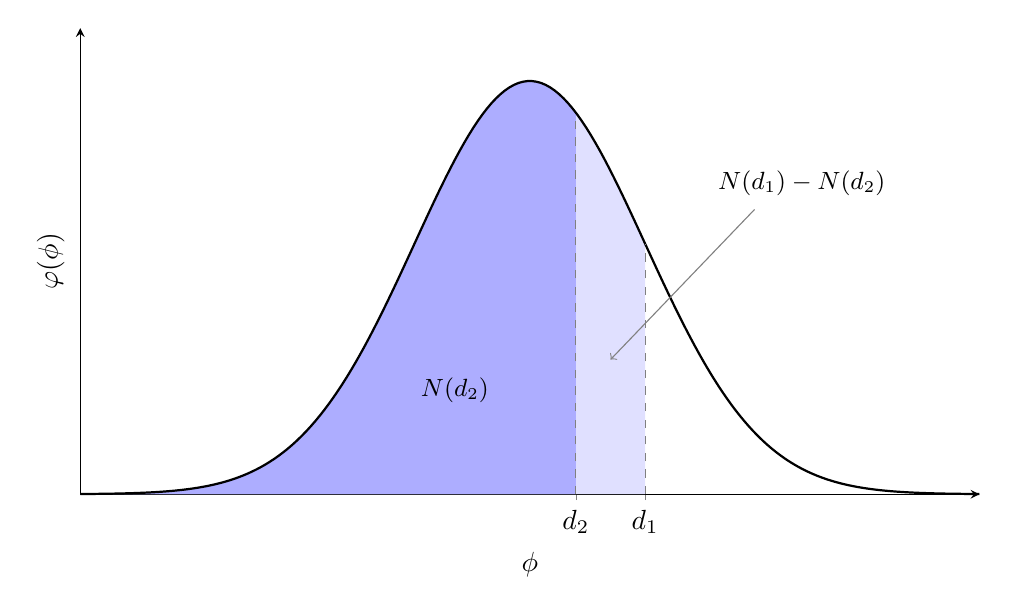
\begin{tikzpicture}
\begin{axis}[
  width=13cm, height=7.5cm,
  samples=200,
  axis lines=left,
  xlabel={$\phi$},
  ylabel={$\varphi(\phi)$},
  xmin=-3.9, xmax=3.9,
  ymin=0, ymax=0.45,
  xtick={0.4,1.0},
  xticklabels={$d_2$,$d_1$},
  ytick=\empty,
  clip=false,
]
\addplot[domain=-3.9:1.0, draw=none, fill=blue!12]
  {1/sqrt(2*pi)*exp(-x^2/2)} \closedcycle;
\addplot[domain=-3.9:0.4, draw=none, fill=blue!32]
  {1/sqrt(2*pi)*exp(-x^2/2)} \closedcycle;
\addplot[domain=-3.9:3.9, thick, black]
  {1/sqrt(2*pi)*exp(-x^2/2)};
\addplot[dashed, gray] coordinates {(0.4,0) (0.4,0.36827)};
\addplot[dashed, gray] coordinates {(1.0,0) (1.0,0.24197)};
\node[anchor=center] at (axis cs:-0.65,0.10) {\small $N(d_2)$};
\node[anchor=west] at (axis cs:1.55,0.30) {\small $N(d_1)-N(d_2)$};
\draw[->,gray] (axis cs:1.95,0.275) -- (axis cs:0.7,0.13);
\end{axis}
\end{tikzpicture}
\caption{The standard normal density $\varphi(\phi)=\tfrac{1}{\sqrt{2\pi}}e^{-\phi^2/2}$.
The darker area to the left of $d_2$ is $N(d_2)$; together with the lighter strip it
forms the full area to the left of $d_1$, which is $N(d_1)$.}
\label{fig:normal}
\end{figure}

The darker region is $N(d_2)$, the area to the left of $d_2$; under the
risk-neutral measure this is precisely the probability that the call is exercised.
The full shaded region, extending to $d_1$, is the larger area $N(d_1)$. Since
$d_1 = d_2 + \sigma\sqrt{T-t}$ always lies to the \emph{right} of $d_2$, we have
$N(d_1) > N(d_2)$; the thin strip separating them, of width $\sigma\sqrt{T-t}$,
is exactly the difference $N(d_1) - N(d_2)$.

When the option is deep in the money ($S \gg K$), both $d_1$ and $d_2$ are large and
positive: the two vertical lines slide far to the right, almost all of the area is
captured, and $N(d_1), N(d_2) \to 1$, so the price approaches its discounted
intrinsic value $S - K e^{-r(T-t)}$. Conversely, deep out of the money
($S \ll K$), both lines slide far to the left, $N(d_1), N(d_2) \to 0$, and the
option is worth almost nothing.

\section{Summary and Discussion}

Starting from the Black--Scholes partial differential equation and reducing it to
the heat equation, we have obtained in closed form the fair value at time $t$ of a
European call option of strike $K$ and maturity $T$, written on an underlying of
spot price $S$:
\begin{equation}\label{eq:bs-summary}
    V(S,t) = S\,N(d_1) - K\,e^{-r(T-t)}\,N(d_2) 
\end{equation}
where
\begin{align}
  d_1 &= \frac{\ln\frac{S}{K} + \left(r + \tfrac{1}{2}\sigma^2\right)(T-t)}{\sigma\sqrt{T-t}}, \\[4pt]
  d_2 &= \frac{\ln\frac{S}{K} + \left(r - \tfrac{1}{2}\sigma^2\right)(T-t)}{\sigma\sqrt{T-t}}
       = d_1 - \sigma\sqrt{T-t},
\end{align}
and $N(\cdot)$ denotes the cumulative distribution function of the standard normal
law as it has already been mentioned in Section~\ref{sec:bs-pde}.

\subsection*{Risk-neutral valuation}
The fact that the risk-free rate $r$, and not the stock's real expected return, governs the
price above is no accident: it reflects a principle that underlies the whole theory
of derivative pricing, known as \emph{risk-neutral valuation}. The principle states
that, to value a derivative, one may pretend to live in a \emph{risk-neutral world}
-- a hypothetical market in which investors are indifferent to risk and therefore
demand no additional expected return for bearing it. Our own world is plainly not
of this kind: the more risk investors take on, the higher the return they require.
Yet, almost miraculously, the value obtained for an option under the risk-neutral
assumption is identical to the one it has in the real world. This is what makes the
theory workable, as it frees the price from any need to know the risk preferences
of buyers and sellers, which are in practice all but impossible to measure.

Additionally, the fact that an option can be priced without reference to risk aversion seems paradoxical
at first, since options are themselves risky investments. The resolution is that an
option is valued \emph{relative to its underlying}. The risk attitudes of investors
are already embedded in the equilibrium price $S$ of the stock: when investors
become more risk-averse the stock price falls, but the formula expressing the
option price \emph{in terms of} that stock price is left unchanged. The same
mechanism is visible in our own derivation. The delta-hedging portfolio was
constructed to be instantaneously riskless, and in forming it the stock's
real-world drift $\mu$ cancelled, leaving a partial differential equation that
contains $r$ but not $\mu$. Since the drift is the only place where risk preferences
could have entered, the price cannot depend on them.

A risk-neutral world is convenient precisely because two simplifications hold there:
\begin{enumerate}
  \item the expected return on a stock, or on any other asset, is the risk-free rate $r$;
  \item the rate used to discount expected cash flows, from an option or any other
        instrument, is again the risk-free rate $r$.
\end{enumerate}
Under these two rules the call price is nothing but its expected payoff at maturity,
computed under the risk-neutral measure $\mathbb{Q}$ and discounted at $r$,
\begin{equation}\label{eq:rn-expectation}
  V(S,t) = e^{-r(T-t)}\,\mathbb{E}^{\mathbb{Q}}\!\left[\max(S_T - K,\,0)\right]
\end{equation}
and the two terms of our closed-form result are exactly the two halves of this
expectation: $S\,N(d_1)$ is the value of the share received, $K\,e^{-r(T-t)}N(d_2)$
the value of the strike paid, and $N(d_2) = \mathbb{Q}(S_T > K)$ is the
risk-neutral probability that the option is exercised.

\subsection*{Reading the formula}
Each piece carries a financial meaning. Everything hinges on a single event: the
call is exercised only if the stock finishes above the strike, $S_T > K$, and under
the risk-neutral measure $N(d_2)$ is precisely the probability of this happening.
The second term then reads straight off its factors: the holder pays the strike $K$
on exercise, which occurs with probability $N(d_2)$, so $K\,N(d_2)$ is the expected
payment at maturity, and the discount factor $e^{-r(T-t)}$ brings it back to today's money,
making $K\,e^{-r(T-t)}\,N(d_2)$ the value today of the strike the holder expects to
pay. The first term, $S\,N(d_1)$, is its mirror image on the receiving side, the
value today of the share collected at exercise; equivalently, $N(d_1)$ is the
option's \emph{delta}, the quantity of the underlying one must hold to hedge the
option locally. The price is therefore the value of what the holder receives, the
share, minus the value of what they pay, the strike, each scaled by the appropriate
probability. The numbers $d_1$ and $d_2$ measure, in units of the standard
deviation $\sigma\sqrt{T-t}$ of log-returns over the remaining life, how far the
option sits in or out of the money, and differ by exactly that one standard
deviation, $d_1 = d_2 + \sigma\sqrt{T-t}$.

\subsection*{When the formula applies}
The derivation rests on a deliberately idealised market. The option must be
\emph{European}, exercisable only at maturity, and written on an underlying that
pays \emph{no dividends} over the life of the contract. The price $S$ is assumed to
follow a geometric Brownian motion with \emph{constant} volatility $\sigma$ and
\emph{constant} risk-free rate $r$, so that log-returns are normally distributed.
As we have already mentioned in Section~\ref{sec:assumptions}, the market is taken to be frictionless, no transaction costs or taxes, unrestricted
short selling, continuous trading, perfectly divisible assets, and free of
arbitrage. Under these hypotheses the delta-hedging argument is exact and the value
above is the unique no-arbitrage price.

\subsection*{Limitations and modern extensions}
These assumptions are convenient but empirically fragile, and the most fragile is
constant volatility. Real markets display a \emph{volatility smile}: options of
different strikes and maturities trade at different implied volatilities, which a
single constant $\sigma$ cannot reproduce. Returns also show heavier tails and
volatility clustering than a lognormal model permits. For this reason
Black--Scholes is today used less as a literal pricing model than as a common
language, prices are quoted through their implied volatility, and as a benchmark
against which richer models are calibrated.

Those richer models relax the constant-volatility hypothesis by letting the
variance itself evolve randomly. The best known is the \emph{Heston}
stochastic-volatility model, in which the instantaneous variance $v_t$ follows a
mean-reverting square-root diffusion of \emph{Cox--Ingersoll--Ross} type,
\begin{equation}\label{eq:heston-var}
  dv_t = \kappa(\theta - v_t)\,dt + \xi\sqrt{v_t}\,dW_t^{v},
\end{equation}
with $\kappa$ the speed of mean reversion, $\theta$ the long-run variance, and
$\xi$ the volatility of volatility. By correlating the variance shocks $dW_t^{v}$
with the price shocks, this model reproduces the smile and the asymmetry of
observed option prices while remaining semi-analytically tractable. Other common
extensions include local-volatility models, which fit the entire observed surface,
and jump-diffusion models, which add discontinuous moves to capture sudden crashes.
Black--Scholes nevertheless remains the foundation on which all of these are built.

\end{document}